\chapter{\IfLanguageName{dutch}{Algemene resultaten}{Results}}%
\label{ch:resultaten}

\subsection{Doelstelling}
Deze samenvatting presenteert de kernresultaten van het onderzoek uitgevoerd in de bachelorproef, gericht op de ontwikkeling van geavanceerde methoden voor de detectie en classificatie van koeiengedrag in een agrarische omgeving.

\section{Resultaten}
\subsection{Detectie en Classificatie van Koeiengedrag}
Het onderzoek heeft geleid tot de ontwikkeling van een robuust systeem dat in staat is om koeien te detecteren en hun gedrag in real-time te classificeren. Dit wordt gerealiseerd door video-opnamen gemaakt in het veld te analyseren met behulp van een geavanceerd machine learning model, de YOLOv8l. Dit model is specifiek getraind op een zorgvuldig samengestelde en gelabelde dataset, wat resulteert in snelle en accurate gedragsvoorspellingen. De belangrijkste voordelen van dit model zijn de hoge snelheid van beeldverwerking en de verminderde foutmarge in de gedragsclassificatie, cruciaal voor real-time monitoringtoepassingen.
\subsection{Analyse van Skelet-keypoints}
Deze sectie van het onderzoek onthult een van de meest innovatieve doorbraken: het gebruik van het ViTPose model. Dit model, dat is ontwikkeld met behulp van de uitgebreide APT-36K dataset, is geoptimaliseerd om de keypoints van het skelet van elke gedetecteerde koe nauwkeurig te identificeren. Deze keypoints zijn cruciaal, omdat ze gedetailleerde informatie verschaffen over de houding en bewegingen van de koeien.

De gegevens van de keypoints zijn niet alleen nuttig voor het in kaart brengen van de fysieke activiteiten van de koeien, maar zijn ook essentieel voor een diepgaande en gedetailleerde gedragsanalyse. Door nauwkeurig de bewegingen van specifieke lichaamsdelen te volgen, kunnen onderzoekers verfijnde inzichten verkrijgen in het natuurlijke gedrag van de koeien, zoals graaspatronen, rustposities, en interacties met andere koeien.

Bovendien speelt de precisie waarmee deze keypoints worden geïdentificeerd een cruciale rol bij het verifiëren en verbeteren van gedragsclassificaties. Wanneer de keypoints met een hoge mate van zekerheid worden vastgesteld, biedt dit een robuuste basis voor het algoritme om nauwkeurige gedragsclassificaties te maken. Dit is vooral van belang in situaties waar de gedragspatronen subtiel en complex zijn, en waar traditionele detectiemethoden mogelijk tekortschieten.

Het vermogen van het ViTPose model om geavanceerde analyses van koeiengedrag mogelijk te maken, opent nieuwe deuren voor het verbeteren van dierwelzijn en het efficiënt beheren van vee. Dit wordt bereikt door een beter begrip van hun gedragsbehoeften en -reacties op verschillende omgevingsfactoren, wat leidt tot meer gerichte en diervriendelijke managementstrategieën.
\subsubsection{Gedrag matches van pose vs classificatie}
98 procent matches tussen pose en classificatie van gedrag. Dit geeft een hoge mate van betrouwbaarheid aan in de voorspellingen van het systeem. 
Hieruit kan je ook conclusies trekken over de nauwkeurigheid van de pose estimation en de classificatie van gedrag, aangezien deze resultaten sterk overeenkomen.
\newline
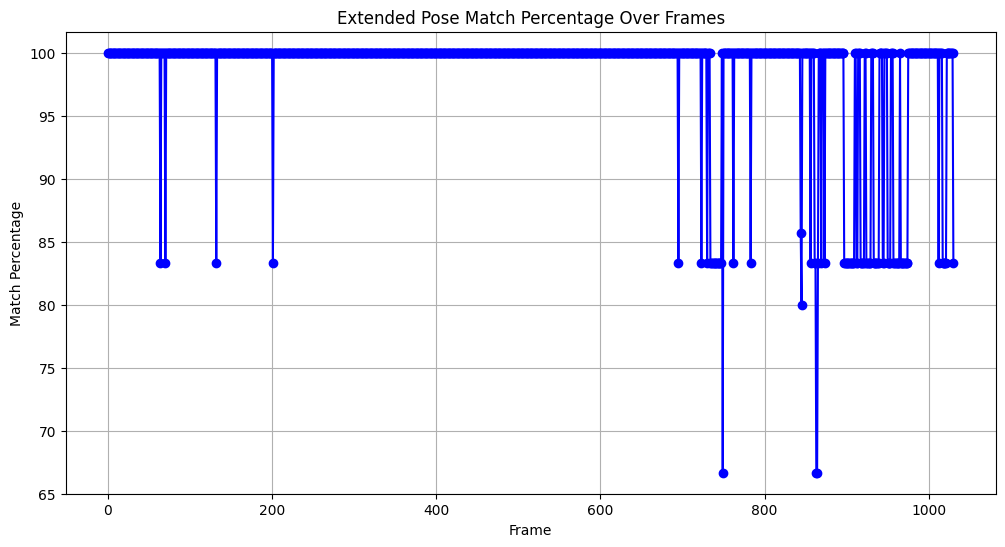
\includegraphics[width=\linewidth]{resultaten_pose_matches.png}
\newline
\subsubsection{Voorbeelden van betere gedragsclassificatie door pose estimation}
Deze afbeeldingen tonen de verbetering in gedragsclassificatie door de diepere analyse van lichaamshoudingen met de pose estimation. (links = classificatie gedrag, rechts = pose estimation gedrag)
\newline
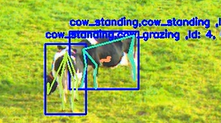
\includegraphics[width=\linewidth]{resultaten_verbetering_pose.png}
\newline
Deze afbeeldingen illustreren hoe de nauwkeurigheid van gedragsclassificatie afneemt door problemen met pose estimation, zoals een slechte positie van de koe. Mijn oplossing houdt in dat als de betrouwbaarheid van de keypoints te laag is, de voorspelling als onbetrouwbaar wordt beschouwd. In dat geval wordt het pose-gedrag niet voorspeld en blijft de oorspronkelijke gedragsclassificatie behouden.
\newline
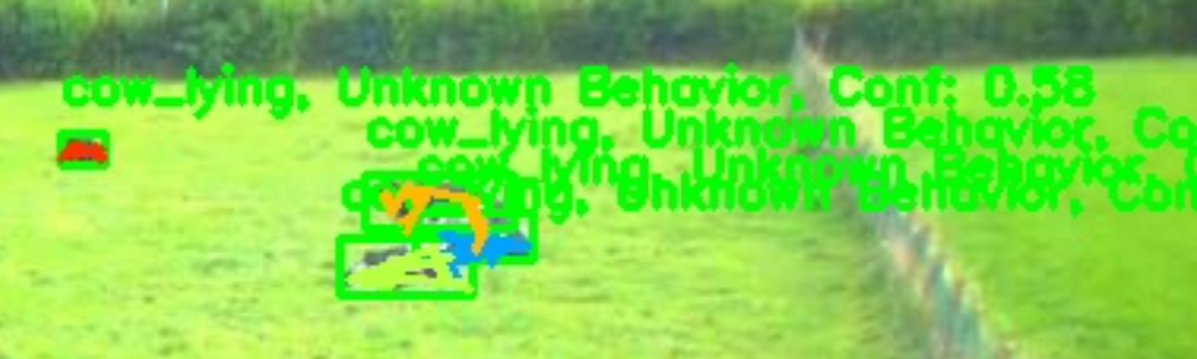
\includegraphics[width=\linewidth]{resultaten_slechte_pose_gedrag.png}
\newline
\subsection{Locatiebepaling via Cameraperspectieftransformatie}
De locatiebepaling van elke koe via cameraperspectieftransformatie vormt een innovatieve uitbreiding van het systeem. Deze techniek, die geavanceerde algoritmen gebruikt om de GPS-locatie van de koe te bepalen op basis van camerabeelden, verhoogt de nauwkeurigheid door integratie van beeldstabilisatietechnieken. Een belangrijk voordeel van deze methode is dat het de noodzaak elimineert om fysieke sensoren of GPS-apparaten direct op de koeien aan te brengen, wat bijdraagt aan een diervriendelijkere benadering van monitoring.

Deze techniek biedt niet alleen een diervriendelijk alternatief, maar verzekert ook continuïteit en betrouwbaarheid in de locatiedata, aangezien er geen risico is op uitval of defecten van sensoren die normaal gesproken op de koeien bevestigd zouden worden. Bovendien is deze methode bijzonder effectief in agrarische gebieden waar traditionele monitoringstechnieken zoals het gebruik van halsbanden of andere vormen van aan het dier bevestigde tracking niet haalbaar of wenselijk zijn.

Door gebruik te maken van deze cameragebaseerde locatiebepaling, kunnen boeren nauwkeurig de locatie en bewegingen van hun vee volgen zonder de welzijn van de dieren in gevaar te brengen. Dit leidt tot beter weidebeheer en geoptimaliseerde veebewegingsroutes, terwijl tegelijkertijd de gezondheid en het comfort van de koeien worden gewaarborgd. Deze aanpak ondersteunt niet alleen een effectiever beheer van het vee, maar bevordert ook een meer ethisch verantwoorde veehouderij.
\section{Conclusie}
De combinatie van deze technologieën biedt een nauwkeurige methode voor het lokaliseren en classificeren van het gedrag van koeien, wat een significante verbetering betekent voor het beheer en de monitoring van vee in de landbouw.
\newline
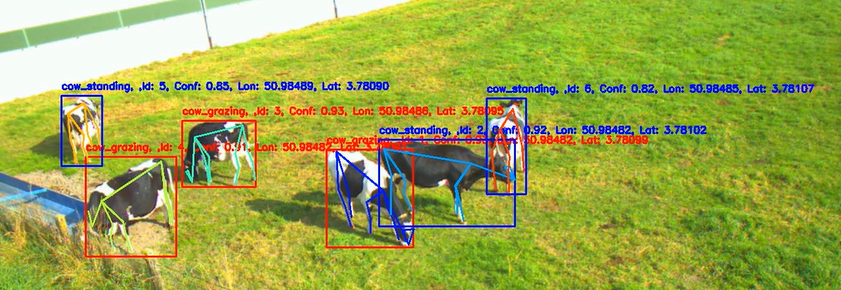
\includegraphics[width=\linewidth]{resultaten_alles.png}
\newline